%%%%%%%%%%%%%%%%%%%%%%%%%%%%%%%%%%%%%%%%%%%%%%%%%%%%%%%%%%%%%%%%%%
%%%%%%%% CPSC 66 SPRING 2021  REPORT %%%%%%%%%%%%%%%%%%%%%%%%
%%%%%%%% This template is modified from ICML 2014 %%%%%%%%%%%%%%%%
%%%%%%%%%%%%%%%%%%%%%%%%%%%%%%%%%%%%%%%%%%%%%%%%%%%%%%%%%%%%%%%%%%

\documentclass{article}

%include any external packages here.  This is similar to loading a
%library in python or C++

% use Times
\usepackage{times}
% For figures
\usepackage{graphicx}
\usepackage{subfigure}
% \usepackage{caption}
% \usepackage{subcaption}

% \usepackage{subfig}

% For citations
\usepackage{natbib}

% For algorithms and pseudocode
\usepackage{algorithm}
\usepackage{algorithmic}

%Adds hyperlinks to your citations automatically
\usepackage{hyperref}

% Packages hyperref and algorithmic misbehave sometimes.  We can fix
% this with the following command.
\newcommand{\theHalgorithm}{\arabic{algorithm}}

\usepackage[accepted]{icml2014}


% If your title is long (below), use this command to also provide
% short version.  This will go on the top of every page
\icmltitlerunning{Final Report}

\begin{document}

\twocolumn[ %use two column if you need a text to span across the whole page
\icmltitle{ CPSC 66 Final Report: \\ % \\ force a new line
At War with WAR: Using Machine Learning to Evaluate a Baseball Player's Contribution to Their Team}

\icmlauthor{George Briggs}{gbriggs1@swarthmore.edu}
\icmlauthor{Matthew Loomis}{mloomis1@swarthmore.edu}
\icmlauthor{Otis Peterson}{opeters1@swarthmore.edu}

\vskip 0.3in
]

\begin{abstract}
In this study, we will analyze various baseball team statistics from the 1947 to 2015 MLB seasons. We use linear regression and random forest regression models to determine which statistics for batter most strongly correlate with winning percentage for teams. Once we have these machine learning models trained, we applied the models to individual players, as a way to establish a comprehensive ranking between players. Furthermore we extended this project to apply a similar method to pitchers, finding that the accuracy of these models was much higher than the accuracy of the models trained on just the batting statistics. We then further extended the project to evaluate the player rankings compared to the salary they were paid, to identify potentially overpaid or underpaid batters.
\end{abstract}

\section{Introduction}
\label{introduction}

	Millions of people call themselves fans of Major League Baseball, the MLB. The MLB employs over a thousand players, each with a slew of statistics based on their performance. Thus, the natural question arises: how do we rank or assign value to baseball players based on their stats? This question, while a fun dinner-table discussion for fans, also holds real value for owners of different MLB teams, who must decide which players are worth buying, and how much to pay them as well. Additionally, if an MLB player knows that they’re getting underpaid, they might be able to use the model to provide good evidence for an increase in pay. In this paper we seek to answer this question using various machine learning techniques that will provide a comprehensive ranking of baseball players.
	
	If you know much about baseball statistics you’ll be thinking about WAR right now. WAR, standing for wins above replacement, attempts to calculate the number of wins a baseball team gets by having that player, compared with if they had an average replacement level player take their place. Generally, a WAR between 1-2\cite{war} is an average player, while anything above 6 is considered remarkable. 
	
	WAR is a remarkably complex statistic that can take into account the hits you generate, your speed on the basepaths, and the runs you prevent defensively. To further complicate things, there isn’t only one way to calculate it. fWAR, bWAR, and WARP are all different ways to calculate WAR that different organizations have come up with. The nuances of this could be a paper of its own, and we encourage you to look into this more if you’re interested. But all this begs the question: given that so many different ways to calculate WAR exist, what can we add by doing more research into the field?
	
    We hope to provide a machine learning point of view that has not yet been considered. Specifically, we would do this through techniques such as linear regression and random forest regression. While previous WAR calculations are complex, they also feature some arbitrarily selected constants that likely have room for improvement. While this research will likely not immediately strike gold with the perfect player ranking statistic, it will ideally work towards the integration of machine learning into the WAR/player ranking narrative.

\section{Methods}
\label{methods}

\subsection{Linear Regression}
\label{linearreg}

The primary model that we used for the project was linear regression.  Linear regression requires virtually no hyperparameters and instead picks weights for each of the feature variables such that it minimizes the sum of squared errors. While it can be slow when run on inputs with an abundance of parameters, for the given project we had no issue with that. The primary reason that we chose linear regression is that it’s one of the simplest models that we have for regression tasks. By simply assigning a coefficient to each feature variable directly we can get a good sense of which statistics are most important to maximize, as our goal is to maximize the winning percentage. 

This simplicity comes at a cost, however. As it is a simple model, it often fails to capture nuance in data, assuming linearity when that may not be the case. Furthermore, it can often be led astray by noise, and is prone to overfitting. Despite this, as shown later, linear regression had the higher accuracy rating of the two models.

\subsection{Random Forest Regression}
\label{randomforest}

The second model we chose to use for the project was Random Forest, which is an ensemble learning algorithm that is used mainly for classification and regression problems. The Random Forest algorithm is unique because it uses many decision trees in its classification and regression processes. Because it utilizes numerous decision trees, the algorithm needs to find a way to create diversity between the individual trees. To do this, the algorithm bootstraps the training data set using a process called bootstrap aggregation to resample the data set rows and also varies the amount of available features that can be used by each decision tree. This subsampling is an effective tool for the algorithm because it allows for an increased diversity of the models which results in more independence and less overfitting of the ensemble.

The algorithm contains two hyperparameters, the first being the total number of decision trees that are being used. The second hyperparameter, commonly referred to as ‘f’, represents the number of available features that each tree uses. A large value of f tends to decrease diversity and increase accuracy while a small value of f increases diversity and decreases accuracy. 

Once the data set is resampled, each decision tree makes a prediction based on its given data. For classification problems, the Random Forest algorithm takes the most commonly predicted decision of all the trees for its final prediction, while regression problems take the average of all the tree predictions for its final prediction point.

\subsection{KNN Regression}
\label{randomforest}

The third model we used was KNN regression. KNN regression is a non-parametric method, meaning that it does not specify a distribution shape. Our KNN algorithm uses the euclidean distance formula $ d(x,y) = \sqrt{\Sigma_{i=0}^n(y_i - x_i)^2}$ to obtain the ‘neighborhood’. This neighborhood contains the $k$ nearest points in the dataset to the independent variable whose dependent variable we are attempting to predict. Our algorithm is then able to create a prediction for the dependent variable by averaging the dependent variables contained in our neighborhood.

\section{Main Stat Generation}
\label{mainstat}

    \subsection{Experiments}
    \label{experiments1}
    
When using our data, there was a number of pre-processing/manipulation that we did to make the data usable. The individual players had the following stats: player ID (pID), the year played (yID), Games played (G), at bats (AB), runs scored (R), hits (H), doubles (2B), triples (3B), home runs (HR), runs batted in (RBI), stolen bases (SB), times caught stealing (CS), walks (BB), strikeouts (SO), intentional walks (IBB), times hit by pitches (HBP), sacrifice hits (SH), sacrifice flies (SF), and times grounding into a double play (GIDP). Teams had many similar stats, but some discrepancies. Notably, teams included some pitching statistics and fielding percentage (FP) (which were irrelevant for the purpose of batting ability), and winning percentage (our target).

First, it’s worth noting the stats that we decided to drop. Clearly unique/non-numeric identifiers of players and teams needed to be dropped as non-numeric values wouldn’t work with the regressors, and even more so, unique values are always unhelpful when performing machine learning, allowing the models to overfit to the training set, learning no generalizability. We also chose to drop Rs and RBIs because these stats, while they did greatly improve the “accuracy” of the model, they depend too much on other players on the team. For example, you can’t be given the opportunity to drive in a run and record an RBI if the batters ahead of you in the lineup aren’t able to get on base. We also chose to omit errors committed/fielding percentage. This, while potentially a good indicator wasn’t possible within the scope of the project\footnote{The FP for players was instead listed as the number of errors. This means if we wanted to incorporate FP we would have had to find an entirely dataset to accurately use this information}. Finally, some stats were dropped from the player’s dataset that may have been helpful in predicting efficacy, but just weren’t present in the team’s dataset, including IBB or GIDP. 

We also took techniques to remove outliers in two key ways. First, we trimmed our dataset to just include players/teams in the years after 1947, post-integration era. This is a common technique when performing analysis on baseball statistics. Many early games are poorly recorded, in addition to being played in very different ways than modern baseball. This bound on the years limits the effect that the year of recording the data plays on our model. Second, when ranking players we made sure to only include batters that had 150 or more ABs. This limited the effect of a player that, say, only went to bat once, but hit a home run. These outliers could clearly cause issues in the ranking/normalization process described later.

Finally, we simplified our data by turning the H stat into the amount of singles hit (1B). Because H = 1B + 2B + 3B + HR, by subtracting out the 2Bs, 3Bs, and HRs from the H category we’re left with H, thus removing collinearity. 

Thus, the stats that we ended up training on were 1Bs, 2Bs, 3Bs, HRs, BBs, SOs, CSs, and SBs. Furthermore, we first divided each of the stats based off of the number of ABs recorded. This was simply to make sure that, say, the number of HRs a player got was related to the number of opportunities a player had to hit HRs. Finally, we normalized each of the stats to make them all between 0 and 1, based on the minimums and maximums of the dataset.

Other more advanced stats are often used when analyzing a baseball player’s batting ability, such as OBP, OPS, BABIP, and more. However, because all of the advanced stats are different ways to manipulate the simple stats that we’re already using, we opted to omit advanced stats, as all it would do is add more collinearity and overrepresentation of data.

Once our dataset was prepared, we began to train our models. In order to test for accuracy, we did a train/test split on the teams, fit the model to the training data, and calculated the accuracy on the testing data. However, in order to construct the model that we used to rank players we fit the model to all of the teams. The increased amount of data theoretically allows for a more comprehensive and accurate model. This doesn’t cause any issues when testing, because this model is only used to establish rankings for players, who don’t have any winning percentage associated with them to begin with. In other words, the model is still being “tested” on data it hasn’t seen before, thus not breaking the cardinal rule of machine learning.

    
    \subsection{Results and Discussion}
    \label{results1}
    
    After running the linear regression and random forest regressors on the data, we were able to output the top ranked players based on our models. The two models showed a lot of similarities, both listing Barry Bonds 2002, 2004, and 2001 season as their top 3. Other notable players included Rickey Henderson, Willie Mays, and Hank Aaron: some of the all time greats\footnote{The full rating is available with our code, or contact us for help}. When calculating the accuracy of the models linear regression and random forest scored at .286 and .235 respectively. The linear regression model found the weights in figure \ref{fig:weights}. These make sense as, broadly, hits are weighted positively, and negative things like strike-outs are ranked negatively.
    
    
        
    \begin{figure}[h!]
    \begin{center}
      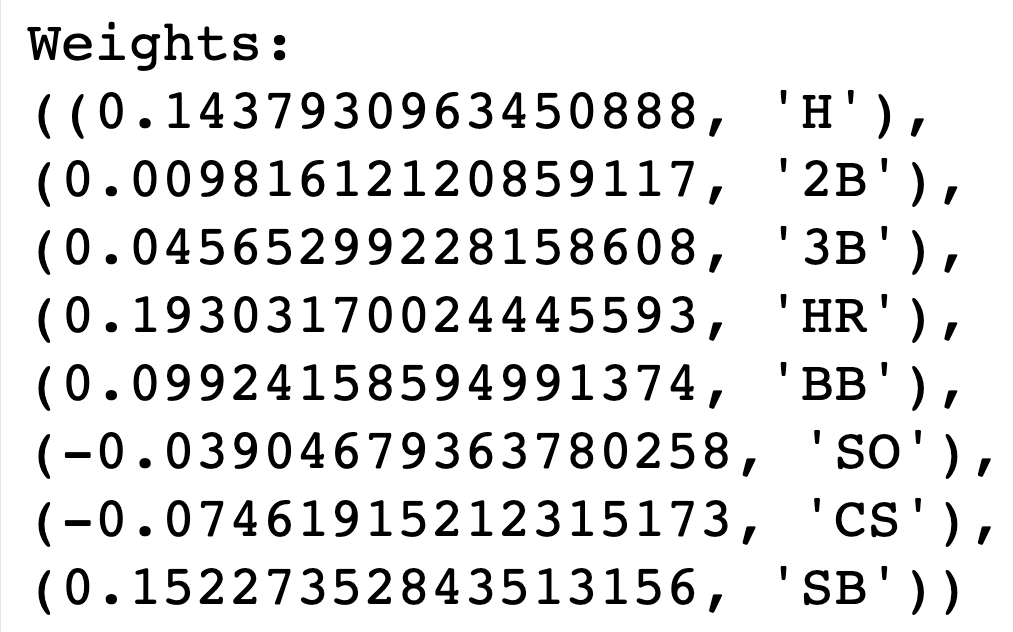
\includegraphics[scale=.105]{weights.png}
      \end{center}
      \caption{Weights for linear regression model}
      \label{fig:weights}
    \end{figure}
    
    In figures \ref{fig:lr_acc} and \ref{fig:rf_acc}, we plot the predicted winning percentage against the true winning percentage, where in a perfect world all data would fall exactly on the y=x line.
    
\begin{figure}[!tbp]
  \centering
  \begin{minipage}[b]{0.4\textwidth}
    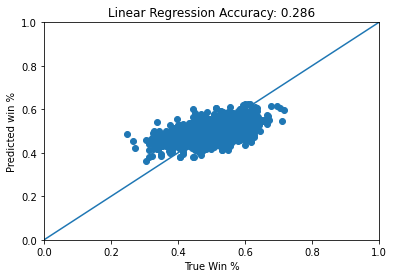
\includegraphics[width=\textwidth]{lr_acc.png}
    \caption{Linear Regression Model}
    \label{fig:lr_acc}
  \end{minipage}
  \hfill
  \begin{minipage}[b]{0.4\textwidth}
    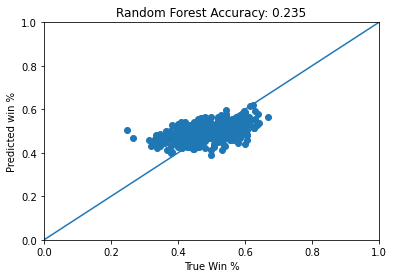
\includegraphics[width=\textwidth]{rf_acc.png}
    \caption{Random Forest Model}
    \label{fig:rf_acc}
  \end{minipage}
\end{figure}


While both models do okay, they both fail in a fairly large way. Ultimately, the model struggles to predict low/high win percentage teams, and attempts to group them all into a roughly similar range of between .4 and .6. The random forest classifier does this more, grouping more of the points closer in that range. Because of this, it makes more sense to use the linear regression model as it provides a more diverse range of scores. Despite the low accuracy ratings, this is an acceptable result for the purpose of this study. A team’s win percentage relies in large part on the team's pitching ability as well as their batting ability. Because we only take into account batting ability here, it makes sense that the models would struggle. 

\textbf{Comparison to Baseball Reference WAR}

Now that we have a comprehensive rating of the players, we can model our ratings against an already established baseball rating, Baseball Reference WAR. 

The scatterplots in figure \ref{fig:war} show a mostly positive linear correlation, which is a good thing. One thing that’s interesting to note is the outliers that we ranked very highly, but WAR ranked more mediocrely. Specifically, Manny Ramirez in 2008, was in the top 25 ranked players, but bosted a mediocre WAR between 2 and 3. This is likely because Manny Ramirez was a poor defensive player, which is something that our model doesn’t consider.

    \begin{figure}[h!]
    \begin{center}
      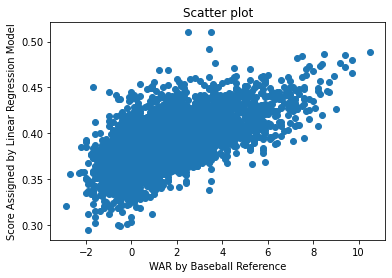
\includegraphics[scale=.5]{war.png}
      \end{center}
      \caption{rWAR plotted against our rankings, 2005-2015}
      \label{fig:war}
    \end{figure}



\section{Extension 1: Salary Prediction}
\label{salary}

    \subsection{Experiments}
    \label{experiments2}
    
    For our salary extension, we are interested in analyzing how our value assignments of players, as measured by our regression model scores, compare to the value assignments assigned by the MLB managers, as measured by the salaries given to their players. To make this comparison, we will use the KNN Regression and Linear Regression algorithms to create a salary prediction based on a player's score. 

	The first step in this process was importing a dataset which included our player salaries as well as the corresponding player IDs. We then merged this dataset with our dataset containing player scores by matching the playerID and yearID of rows in our two datasets. During this process we dropped any rows which did not contain exactly one salary value for the corresponding player and year. The salary dataset only contained entries starting from the year 1985, so we had to drop every row from the player score dataset from before this year. This left us with a data set containing variables: yearID, playerID, score, and salary.
	
	Our next step was to apply our algorithms to our new dataset to create a salary prediction based on player score. In order to increase accuracy, account for inflation, and changes in the MLB salary cap, we controlled for the year when running our KNN Regression. Because our original player score dataset does not include players with less than 150 At Bats and because we are now controlling for the year, we are left with a much smaller pool of data - about 290 players per year on average.
	
    First we used a KNN Regression because it excels in low dimensional datasets (our dataset was one dimensional because our target value only contained player scores). As a result of our limited data, we chose a rather low value for k at 10. This allows us to avoid overfitting while also giving us more variance. Similarly, we also implemented a Linear Regression to determine the strength of the relationship between player score and salary.
    
    \subsection{Results and Discussion}
    \label{results2}
    
    Our models’ salary assignments produced interesting results not because of how well they aligned with the MLB salary assignments, but because of how they differed. Our average coefficient of determination, $R^2$, for our KNN regression model across the 25 seasons we tested, was 0.047, indicating that there is a weak relationship between our value assignment and the MLB’s. Similarly, our Linear Regression model had a very similar correlation coefficient at 0.097, indicating an only slightly stronger relationship. These results are in large part due to our model tending to choose salaries towards the middle of the distribution whereas the actual salaries are spread across a much greater range. 
    
        \begin{figure}[h!]
          \begin{center}
            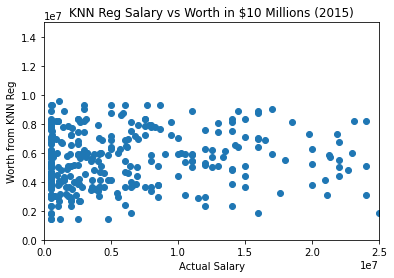
\includegraphics[scale=.5]{knn_salary.png}
          \end{center}
          \caption{Actual Vs Predicted Salary for KNN}
          \label{fig:knn_sal}
        \end{figure}

        \begin{figure}[h!]
          \begin{center}
            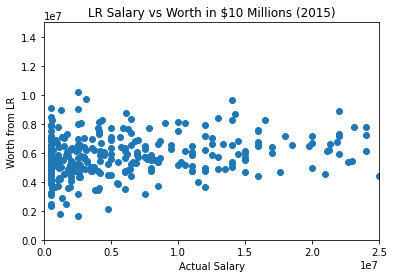
\includegraphics[scale=.5]{lr_salary.png}
          \end{center}
          \caption{Actual Vs Predicted Salary for Linear Reg}
          \label{fig:lr_sal}
        \end{figure}


    As can be seen by figures \ref{fig:knn_sal} and \ref{fig:lr_sal}, our model tends to choose much more moderate salaries for players while the MLB has the majority of the players valued relatively low with a strong rightward skew. Given the roughly normal distribution of our model, observed in the figures, it makes sense that our model tended to choose salaries towards the middle. Ultimately what these findings reveal, is that there is much less variation in what a player is actually worth than indicated by the large variation seen in MLB salaries. In particular, very few of the highest paid MLB players contribute to their team as much as their salary would indicate and nearly all of the lowest paid players are contributing more than their salary would indicate. 


\section{Extension 2: Pitcher Ranking}
\label{pitcher}

    \subsection{Experiments}
    \label{experiments3}
    
    The purpose of adding the pitcher extension to our project was to compare and contrast the pitcher model outputs to the outputs of the hitter model that we created for the main part of the project. To do this, we followed a very similar structure to that of the hitter model, using both linear regression and random forest regression to create model weights for individual pitching statistics and then using those weights to find a correlation to a teams overall winning percentage.
    
    The pitcher data set contains over 35 class labels, each representing a different pitching statistic, so the most difficult part of the data cleaning process was determining which statistics made the most sense to include in our model. We decided to look only at statistics in which the pitcher had the most control over, and came up with a list of five statistics that we used in our model. The list includes earned runs, hits, walks, hit batsmen, and strikeouts. 
    
    \subsection{Results and Discussion}
    \label{results3}
    
    After normalizing the statistics we used our cleaned data set to train our logistic regression model, which had an accuracy of .7708 and gave us associated weights for each of our five imputed pitching statistics. These values are listed below:
	
	BB (walks): -1.2742, Hits (H): -1.8810,  Earned Runs (ER): 3.0065, Strkeouts (SO): 0.00611,  Hit by Pitch (HBP): -2.67
            
    The most notable result after running the pitching data is the large improvement in the overall accuracy of the model (77 percent vs 28.6 percent). This increased accuracy can be attributed to the earned run statistic, which carries the most weight of any hitter or pitcher statistic that we tested. In fact, when the earned run statistic is taken out of the model completely, the accuracy is about 10.5 percent.
    
    When thought of in the context of baseball, it makes sense that the earned run statistic carries so much weight, as runs are the measure of wins and losses in the sport. Thus, if a team is using pitchers that allow fewer runs per inning than their opponents, they are going to be much more likely to win the game. The importance of the earned run statistic also suggests that pitchers are the most important factor in determining the outcome of a game. 


\section{Conclusions}
\label{conclusion}

In this project we provided a machine learning perspective on the complex and highly contested baseball statistic WAR. We used linear regression to calculate weights for the most relevant hitting and pitching statistics, used linear and random forest regression to rank individual player seasons, and used both knn and linear regression to predict and evaluate player salaries. In doing this, we found which hitting and pitching statistics were most correlated with winning and losing games, generated a comprehensive list, ranking all players from the 1947 to 2015 seasons using two different forms of regression, and analyzed the monetary value of players based on their weighted statistics.

The stakeholders for this project include baseball players, coaches, owners, and fans. The following paragraphs will briefly describe the implications for each.

Baseball players are the most widely affected group by our project and WAR analysis in general. On one hand, an emphasis on WAR is great for players that grade out well and rank highly, as it provides these players with more bargaining power and gives them the ability to demand a higher salary during contract negotiations. However, on the other hand, the opposite is also true. Players who do not grade well or are ranked low in WAR analysis would see decreased bargaining power, lower salaries, and potentially a demotion in favor of a player with a higher WAR.

Coaches and owners are a group that can greatly benefit from this project. Our project provides insight into what makes players and teams successful, which is information that can be very useful for owners who want to construct winning teams and for coaches who want to put their players in the best opportunities for success. Our project would also be very useful for owners and general managers during the free agency period, as they can sign players for team-friendly contracts with players that are demanding salaries that are less than their WAR calculated market value. This would help teams keep their budgets within reason while also putting a good roster together.

The fans are the final group that can be affected by this project. There is no doubt that the style of Major League Baseball games change when front offices put an emphasis on WAR and other advanced baseball statistics. This can be easily seen in recent years, where front offices have put on emphasis on acquiring power hitters that hit a lot of homeruns that also strike out a lot, which can make games very boring for fans.   


\section{Further Research}
\label{further}

We have identified several possible future extensions which we believe could be valuable and enlightening additions to our results. For instance, including defensive statistics and controlling for the player positions in our linear regression and random forest regression models could create a more comprehensive scoring index. Taking this idea one step further, it would be beneficial to consult with experts to determine if there are further stats that we could benefit from including. This could also explain some of our deviance from WAR and the lack of correlation between our salary assignments and the MLB’s. Another extension we believe could be very valuable is regressing a player’s success in the MLB (measured by their player score) on their highschool/college statistics. Somewhat similarly, we discussed the possible extension of using age, position, and current player score to predict how a player’s score will change in future seasons. These predictive estimates could have a high utility in giving MLB teams a competitive edge in their decision making. Finally, we could further solidify our findings by using more regression models, such as Gradient Descent, and tuning more of our hyperparameters to reduce bias and variance.


\section*{Acknowledgments}

We would like to thank Ameet Soni and Benjamin Mitchell, who both taught and guided us as we explored the topics of machine learning for the first time.
We would also like to thank Swarthmore College and the entire Computer Science department for employing these two professors, and allowing us to take this course during truly unprecendented times.

% In the unusual situation where you want a paper to appear in the
% references without citing it in the main text, use \nocite
\bibliography{references}
\bibliographystyle{icml2014}

\end{document}
